\chapter{Introduction}

\section{Overview}

In the field of computational neuroscience, there exist a class of problems relating to mapping the neuron-level structure of the brain. For instance, one might want to precisely model the neural connectivity of an abnormal mouse brain, or observe the connectivity and topology of a worm at different stages of its development. Conventionally, the structure of the brain is inferred from images, whether they are thin slices of a brain imaged with an electron microscope, volumetric images acquired using digital radiograhpy systems (i.e. fMRI, CAT, etc), or visible-spectrum video of exposed brain tissue. Although these imaging technique generate information at different resolution levels, they invariably present a huge data problem: when researchers are presented with small-scale image data, it is fundamentally infeasible to efficiently infer the connectivity and structure of a small cluster of neurons by hand, let alone an entire brain or nervous system, simply because the amount of neurons in a brain is too large.

Many attempts have been made to automate the process of inferring connectivity and topology from images using various algorithmic and machine learning models. In the past five years or so, many of the most successful attempts at this class of problems have utilized Convolutional Neural Networks (CNNs) to achieve their high performance. The goal of this year-long project is to explore many of the different CNN-based approaches that have gained recognition in the past few years in several sub-problems, evaluate their performance and enumerate their deficiencies, and attempt to design new architectures that achieve improved performance in these sub-problems. In addition to increasing performance on established benchmarks, we also make contributions on new sub-problems for which there are no established benchmarks.

\section{Sub-Problems}

The motivation for the research in this field is to better understand the connectivity of neural tissue. Since this is such a broad goal, it stands to reason that there a number of intermediary sub-problems that can be tackled to learn about connectivity. Several of the sub-problems have been heavily studied, and various public competitions have been organized that provide labeled training data and unlabled test data, encouraging competitors to achieve maximum performance against a certain benchmark. As we developed our models, we submitted their predictions to several of these open competitions, often performing well.

% Get rid of this eventually
\medskip

\subsection*{2D Boundary Detection for EM Images}

One of the more established problems in the field is 2D Boundary Detection. The problem statement is such: given a 2-dimensional single-channel (i.e. greyscale) image of neural tissue taken with an electron microscope, produce an image that labels the boundaries of all the distinct cells in the image. An example of this boundary-detection task can be found in Figure \ref{fig:isbi_example}. This task is made particularly difficult by the existence of organelles with well-defined borders, as well as blood vessels and structured interstitial tissue.

\begin{figure}[h]
    \centering
	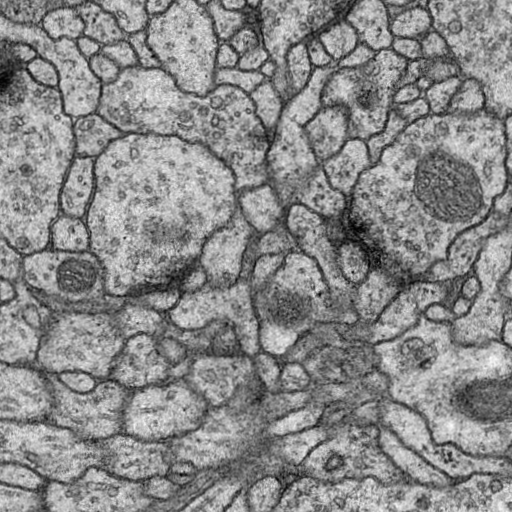
\includegraphics[width=0.33\textwidth]{img/isbi_raw_example}
	\hspace{1cm}
	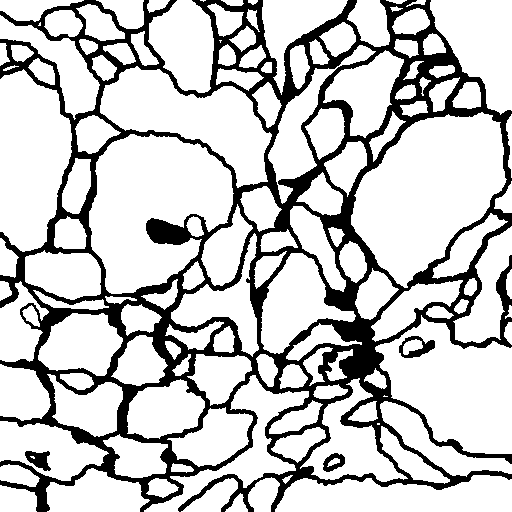
\includegraphics[width=0.33\textwidth]{img/isbi_label_example}
    \caption{An example of 2D boundary detection. Left: the original image taken with an electron microscope. This particular example is neuron tissue taken from \textit{Droposphila melanogaster} in a dataset created for the ISBI 2012 EM segmentation challenge \cite{Arganda-Carreras2015}. The resolution of each pixel is 4nm x 4nm. Right: The ground truth boundaries corresponding to cell membranes in the input image, as labeled by human experts. The labels are binary values, although the actual border deliniation is somewhat arbitrary due to the fact that real applications of boundary detection are invariant to small differences in boundary shapes.}
    \label{fig:isbi_example}
\end{figure}

One prominent competition that evaluates performance on this sort of task is the International Symposium on Biomedical Imaging (ISBI) EM Segmentation Challenge, which has had active submission since 2012. The ISBI Challenge organizers provides a training set of EM images, along with a set of binary boundary maps. The challenge website describes the training data as \quotes{a set of 30 sections from a serial section Transmission Electron Microscopy (ssTEM) data set of the Drosophila first instar larva ventral nerve cord (VNC). The microcube measures 2 x 2 x 1.5 microns approx., with a resolution of 4x4x50 nm/pixel}\cite{Arganda-Carreras2015}. This resolution description implies that each pixel represents a 4x4nm patch on the surface of a slice, with each slice being 50nm thick. We build prediction systems using several different architectures, regularization methods, and data transformation techniques. We make several submissions to the leaderboard, ultimately scoring quite competitively.

% Get rid of this eventually
\medskip

\subsection*{3D Segmentation for EM Volumes}

More recently, the sub-problem of automatic 3D Segmentation has emerged as a popular research area. This sub-problem is formulated as such: given a stack of 2-dimensional EM images generated that represent a 3-dimensional volume of tissue (i.e. the images were taken of successive physical slices of tissue), produce a segementation\footnote{A segmentation of an image or a stack of images is defined as producing a label for each pixel in the image or stack of images, where each unique label corresponds to a discrete object in the physical volume.} of the set of images that uniquely labels each discrete entity in the original volume. That is, if a tissue volume contains a neuron that passes vertically through several different slices, then the portions of each slice through which the neuron passes would be labeled with the same identifier. This problem is significantly more complicated than the boundary prediction problem stated before, because it requires an awareness of context in 3 dimensions, rather than 2. Additionally, most EM datasets are anisotropic, meaning that the resolution is not uniform in all directions (specifically, the z-direction perpendicular to the plane of each image is generally dilated). An example of a segmentation can be found in Figure \ref{fig:snemi3d_example}.

\begin{figure}[h]
    \centering
	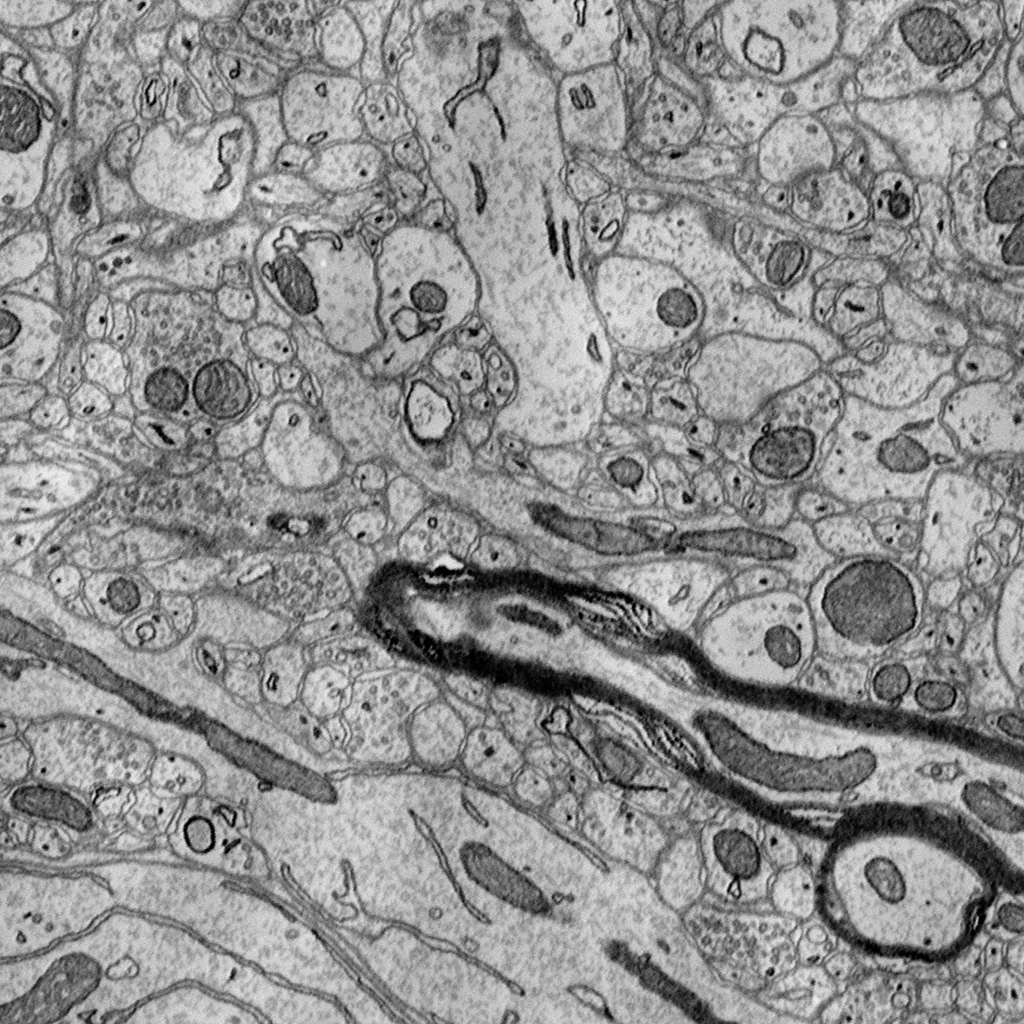
\includegraphics[width=0.33\textwidth]{img/snemi3d_raw_example}
	\hspace{1cm}
	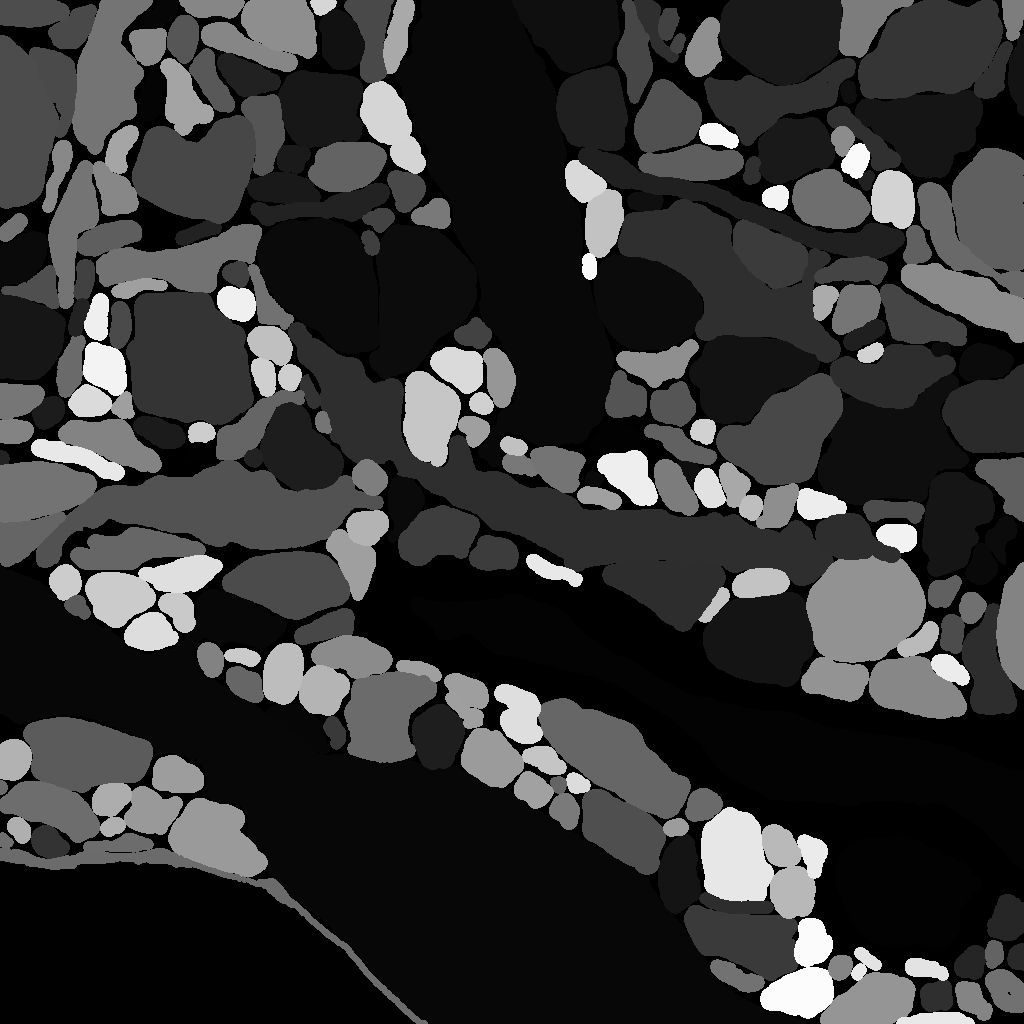
\includegraphics[width=0.33\textwidth]{img/snemi3d_label_example}
    \caption{An example of a 2D cross-section of a 3D segmentation. Left: one of the original images in a stack of images taken with an electron microscope. This particular example is neuron tissue taken from the common mouse in a dataset used in the ISBI 2013 EM segmentation challenge \cite{Kasthuri2015}. The resolution of each pixel is 6nm x 6nm, and each image represents a slice 30nm thick. Right: The ground truth segmentation corresponding to a segmentation of each individual object in the input image, as labeled by human experts. The labels are unique identifiers, although the border deliniation is somewhat arbitrary due to the fact that real applications of boundary detection are invariant to small differences in boundary shapes.}
    \label{fig:snemi3d_example}
\end{figure}

Trivially, the complexity of objects in 3 dimensions is potentially much greater than in two dimensions, so it makes sense that any learning method used to train a system that performs segmentation might be adept at certain types of volumetric data, and inept at others. To evaluate methods on different types of volumetric data, we selected two different challenges that provide us with samples of neural tissue that have different geometric properties, not only due to geometric differences in the underlying tissue but also because of differences in sample preparation techniques. These two challenges are the SNEMI3D Segmentation Challenge and the CREMI Segmentation Challenge.

The SNEMI3D Segmentation Challenge is a highly active challenge (organized in advance of ISBI 2013), and provides a stack of EM images for training, along with ground truth segmentations of the EM images in 3 dimensions. The challenge website describes the training and testing data as \quotes{stacks of 100 sections from a serial section Scanning Electron Microscopy (ssSEM) data set of mouse cortex. The microcube measures 6 x 6 x 3 microns approx., with a resolution of 6x6x30 nm/pixel}\cite{Arganda-Carreras2013}. Like the ISBI 2012 dataset, the SNEMI3D dataset is anisotropic, and particularly dilated in the z-direction. Additionally, the data is from mouse cortex, rather than from \textit{Droposphilia}, and the geometry of the tissue is significantly different. \TODO{Discuss our submissions to this leaderboard.}

The Circuit Reconstruction from Electron Microscopy Images (CREMI) Challenge is a somewhat less-active challenge organized in advance of MICCAI 2016\cite{Funke.Jan2016}. The challenge provides three datasets for training, all of which are volumetric samples of \textit{Drosophila melanogaster}. The training and testing data are stacks of 125 sections from an ssSEM data set, with each slice having a resolution of 4x4x40nm/pixel. These datases are also anisotropic, being dilated in the z-direction. Furthermore, the types of neurons sampled are quite diverse between datasets: from visual inspection, some of the neurites in one of the datasets is much thinner than those in the others, suggesting that models might perform differently when trained/tested on these different datasets. Finally, these datasets are quite a bit noisier than ISBI or SNEMI3D: there are many more major misalignments, many patches of blur, and some slices are missing entirely. These datasets will provide a good measure of how robust our methods are to noise in volumetric data. \TODO{Discuss our submissions to this leaderboard.}

% Get rid of this eventually
\medskip

\subsection*{Image Realignment}

One major hurdle in inferring neural structure from EM images is that the image acquisition process is inherently noisy. While the EM imaging technologies used for the creation of neuron images (typically TEM) are quite stable, there is often variance in sample preparation techniques, resulting in all sorts of distortions and errors at imaging time. One particular type of error, image misalignment, occurs during the slicing of sample tissue, when some physical factor causes a resulting slice to be warped or translated in such a way that the resulting stack of images is misaligned. Intuitively, this means that every point in one EM slice data does not necessarily map to the point directly below it the neighboring slice. An example of slice misalignment can be visualized in Figure \ref{fig:misalignment_example}.

\begin{figure}[h]
    \centering
	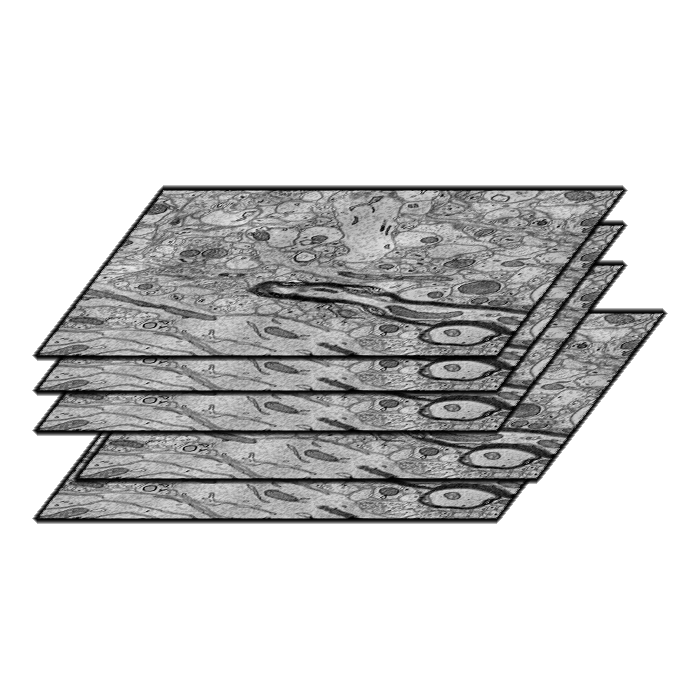
\includegraphics[width=0.33\textwidth]{img/misalignment_example}
	\hspace{1cm}
	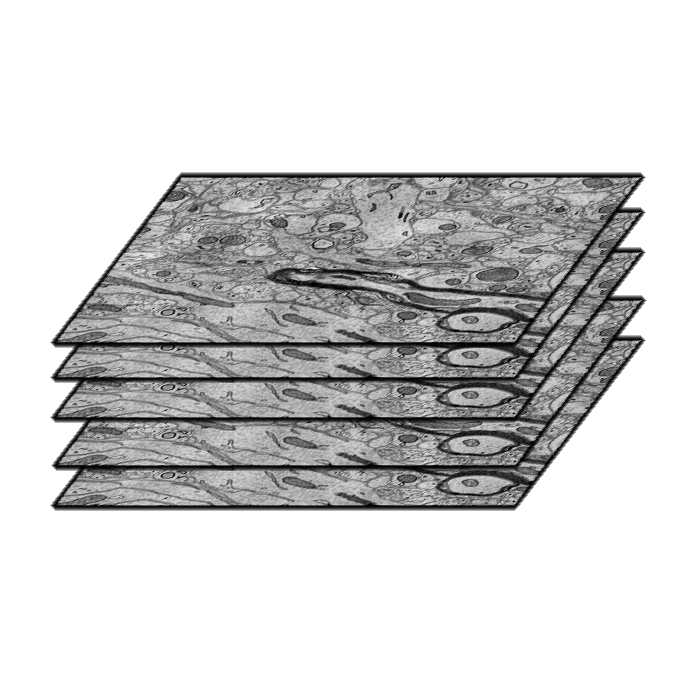
\includegraphics[width=0.33\textwidth]{img/alignment_example}
    \caption{An example of a 3D stack of EM images that contains a misalignment. Left: The provided alignment of a stack. This represents a misalignment where the fourth image in a stack of images actually represents a slice slightly translated in position. Right: The correct alignment of the stack, where all the pixels in the fourth position have been translated enough such that the structures depicted in the input data line up in the z-direction.}
    \label{fig:misalignment_example}
\end{figure}

The problem of misalignment within a set of EM images particularly induces problems in the task of 3D Segmentation. While most techniques are rather invariant to small misalignments (particularly CNNs, which can be trained to be invariant to warping of many kinds), large misaligments can often induce false splitting in segmentations. Very deep CNNs trained with a really diverse set of data would likely be able to compensate for these sorts of misalignments, but it would be more prudent to develop a more efficient strategy for automatically healing misalignments in the data. 

\TODO{There are no current benchmarks or competitions for this task, but we will qualitatively (and quantitatively through downstream tasks) attempt to evaluate our methods on this sub-problem.}